\documentclass[10pt]{article}

\usepackage{icicpe}
\usepackage[utf8]{inputenc}
\usepackage[pdfencoding=auto]{hyperref}
\usepackage{url}
\usepackage{amsmath}
\usepackage{amssymb}
\usepackage{booktabs}
\usepackage{graphicx}
\usepackage{placeins}

\title[english]{When Do Neural Forecasters Help? A Walk-Forward Benchmark on Cryptocurrency Returns and Volatility}

\author[english]{
Gilbert Korir\\
WorldQuant University\\
}

% \finalcopy

\begin{document}

\twocolumn[
\maketitle
\begin{abstract}
Cryptocurrency markets motivate substantial interest in machine learning
forecasting, but many empirical studies rely on single train-test splits,
weak baselines, or validation schemes that risk lookahead bias. We present a
walk-forward benchmark for daily cryptocurrency return and realized volatility
forecasting across BTC, ETH, SOL, BNB, and XRP from 2020--2025. The benchmark
compares naive and historical-mean baselines, ARIMA, XGBoost, LSTM, N-BEATS,
PatchTST, Temporal Fusion Transformer, the zero-shot Chronos foundation model,
and GARCH(1,1) as a volatility-only baseline. Forecasts are evaluated at
one-day and seven-day horizons over 237 asset-splits per target, horizon, and
applicable model using RMSE, MAE, directional accuracy for returns, and
Diebold-Mariano tests with the Harvey-Leybourne-Newbold correction. In the full
benchmark, ARIMA obtains the lowest mean RMSE for one-day returns, Chronos is
marginally best for seven-day returns, and PatchTST obtains the lowest mean
RMSE for realized volatility at both horizons. Directional accuracy for returns
remains close to chance, so these gains should be interpreted as forecast-error
reductions rather than direct trading signals. The results support a calibrated
claim: modern sequence models help most when the target contains persistent
structure, as in realized volatility, and require careful validation before
claims of return predictability.
\end{abstract}

\begin{keyword}
Cryptocurrency forecasting, walk-forward validation, volatility forecasting,
Diebold-Mariano test, time-series foundation models
\end{keyword}
]

\section{Introduction}
Forecasting cryptocurrency markets is difficult because returns are noisy,
heavy-tailed, and non-stationary. Recent work often reports strong performance
from deep learning models, but such claims are hard to interpret when studies
use a single train-test split, tune on future data, or omit strong classical
baselines. This is especially problematic in financial forecasting, where small
validation mistakes can create large apparent gains.

This paper asks a narrow empirical question: under a strictly walk-forward
protocol, do modern neural and foundation models improve on classical baselines
for cryptocurrency returns and realized volatility? The expected answer is not
that deep learning always wins. Rather, we hypothesize that daily log returns
remain close to a random-walk setting, while realized volatility contains more
forecastable structure.

The contribution is a reproducible benchmark that combines expanding-window
validation, classical econometric baselines, modern neural forecasters, a
zero-shot foundation model, and pairwise statistical testing. The resulting
evidence is useful because it separates model novelty from evaluation quality.

\section{Related Work}
Cryptocurrency forecasting has a large and fast-moving empirical literature.
Recent comparative studies report that ensemble and deep learning methods can
outperform conventional models for cryptocurrency price forecasting
\cite{bouteska2024cryptocurrency}, while return-focused work continues to
compare ARMA/GARCH-family models with LSTM and hybrid econometric-neural
approaches \cite{almadany2024forecasting}. Recent volatility studies have also
combined classical volatility models, machine learning, sentiment, and hybrid
decomposition pipelines \cite{brauneis2024crypto,wang2024ceemdan}. At the same
time, recent evidence on cryptocurrency unpredictability cautions that simple
models can remain competitive when evaluation is strictly out of sample
\cite{puoti2025quantifying}.

Time-series foundation models are a parallel development. TimesFM, Lag-Llama,
Chronos, MOMENT, and Moirai show that large pretrained time-series models can
provide useful zero-shot or limited-supervision forecasts across heterogeneous
domains \cite{das2024decoder,rasul2024lagllama,ansari2024chronos,goswami2024moment,woo2024unified}.
Our study connects these two streams by asking whether a zero-shot foundation
model remains competitive on cryptocurrency returns and realized volatility
when evaluated against strong classical, tabular, and neural baselines under a
walk-forward protocol.

\section{Methodology}
\subsection{Data and Targets}
We use daily Yahoo Finance data for BTC-USD, ETH-USD, SOL-USD, BNB-USD, and
XRP-USD from January 2020 to December 2025. For each asset, the return target
is the daily log return,
\begin{equation}
 r_t = \log(P_t/P_{t-1}),
\end{equation}
where $P_t$ is the close price. The volatility target is seven-day realized
volatility, computed as the rolling standard deviation of past log returns. All
lagged features are shifted before rolling aggregation so that time $t$
features use only information available through $t-1$.

\subsection{Validation Protocol}
We use expanding-window walk-forward validation. The initial training window is
730 days. Each split forecasts the next 30 days, then the training window
expands by 30 days. The full benchmark uses all available splits: 48 splits for
BTC, ETH, BNB, and XRP, and 45 splits for SOL, for 237 asset-splits per
target, horizon, and applicable model. Forecast horizons are $h=1$ and $h=7$
days.

\subsection{Models}
The benchmark includes: naive persistence, historical mean, ARIMA(2,0,2),
GARCH(1,1) as a conditional volatility baseline
\cite{bollerslev1986generalized}, XGBoost on lag and rolling features, LSTM,
N-BEATS \cite{oreshkin2020nbeats}, PatchTST \cite{nie2023time}, Temporal
Fusion Transformer (TFT) \cite{lim2021temporal}, and Chronos-T5-small in
zero-shot mode. Because GARCH forecasts conditional volatility rather than
return levels, it is evaluated only for the realized volatility target. Neural
models are trained independently inside each walk-forward split, with all
random seeds fixed.

\subsection{Evaluation}
We report RMSE and MAE for all targets. For returns, we also report directional
accuracy, defined as the fraction of forecasts with the same sign as the
realized return. To compare forecast errors statistically, we use the
Diebold-Mariano test \cite{diebold1995comparing} with the
Harvey-Leybourne-Newbold small-sample correction
\cite{harvey1997testing}. The loss differential is computed using squared
error for the RMSE comparisons. The benchmark follows the forecasting
competition emphasis on comparing diverse model classes under a common
evaluation protocol \cite{makridakis2020m4}.

\subsection{Reproducibility}
All experiments use seed 42 and the configuration in the accompanying
repository. The reported outputs were generated from repository revision
\texttt{abb46b0}. Neural models were trained on Modal A100 workers with
\texttt{max\_steps=1000}; the classical and XGBoost sweep used Modal CPU
workers and completed in approximately 33 minutes. The full benchmark writes
one metrics table and one prediction table, enabling the summary statistics,
rank tables, figures, and Diebold-Mariano tests to be regenerated from saved
forecast outputs. Code, configurations, and seeds will be released in a public
GitHub repository upon acceptance.

\section{Results}
Table \ref{tab:rmse} reports mean RMSE across the full benchmark. The one-day
return task is led by ARIMA, followed closely by historical mean and Chronos.
At the seven-day return horizon, Chronos is marginally best, but historical
mean and ARIMA are nearly tied. This is not evidence that returns are easy to
forecast: directional accuracy remains close to chance, and the return task is
still sensitive to the evaluation protocol. Rather, the result shows that
classical baselines remain hard to beat and that a zero-shot foundation model
can be a strong forecast-error baseline without asset-specific fine-tuning.

\begin{table}[t]
\caption{Best mean RMSE in the full benchmark. Lower is better.}
\label{tab:rmse}
\begin{center}
\begin{tabular}{llcc}
\toprule
Target & Horizon & Best model & RMSE \\
\midrule
Return & 1 day & ARIMA & 0.02226 \\
Return & 7 day & Chronos & 0.03204 \\
Volatility & 1 day & PatchTST & 0.00295 \\
Volatility & 7 day & PatchTST & 0.01075 \\
\bottomrule
\end{tabular}
\end{center}
\end{table}

Figure \ref{fig:rmse} visualizes the full RMSE ranking for each target and
horizon. It highlights the return-volatility contrast: return performance is
clustered among ARIMA, historical mean, and Chronos, whereas PatchTST is most
clearly separated on one-day realized volatility. GARCH is omitted from return
panels because it is a volatility forecaster.

\begin{figure*}[t]
\centering
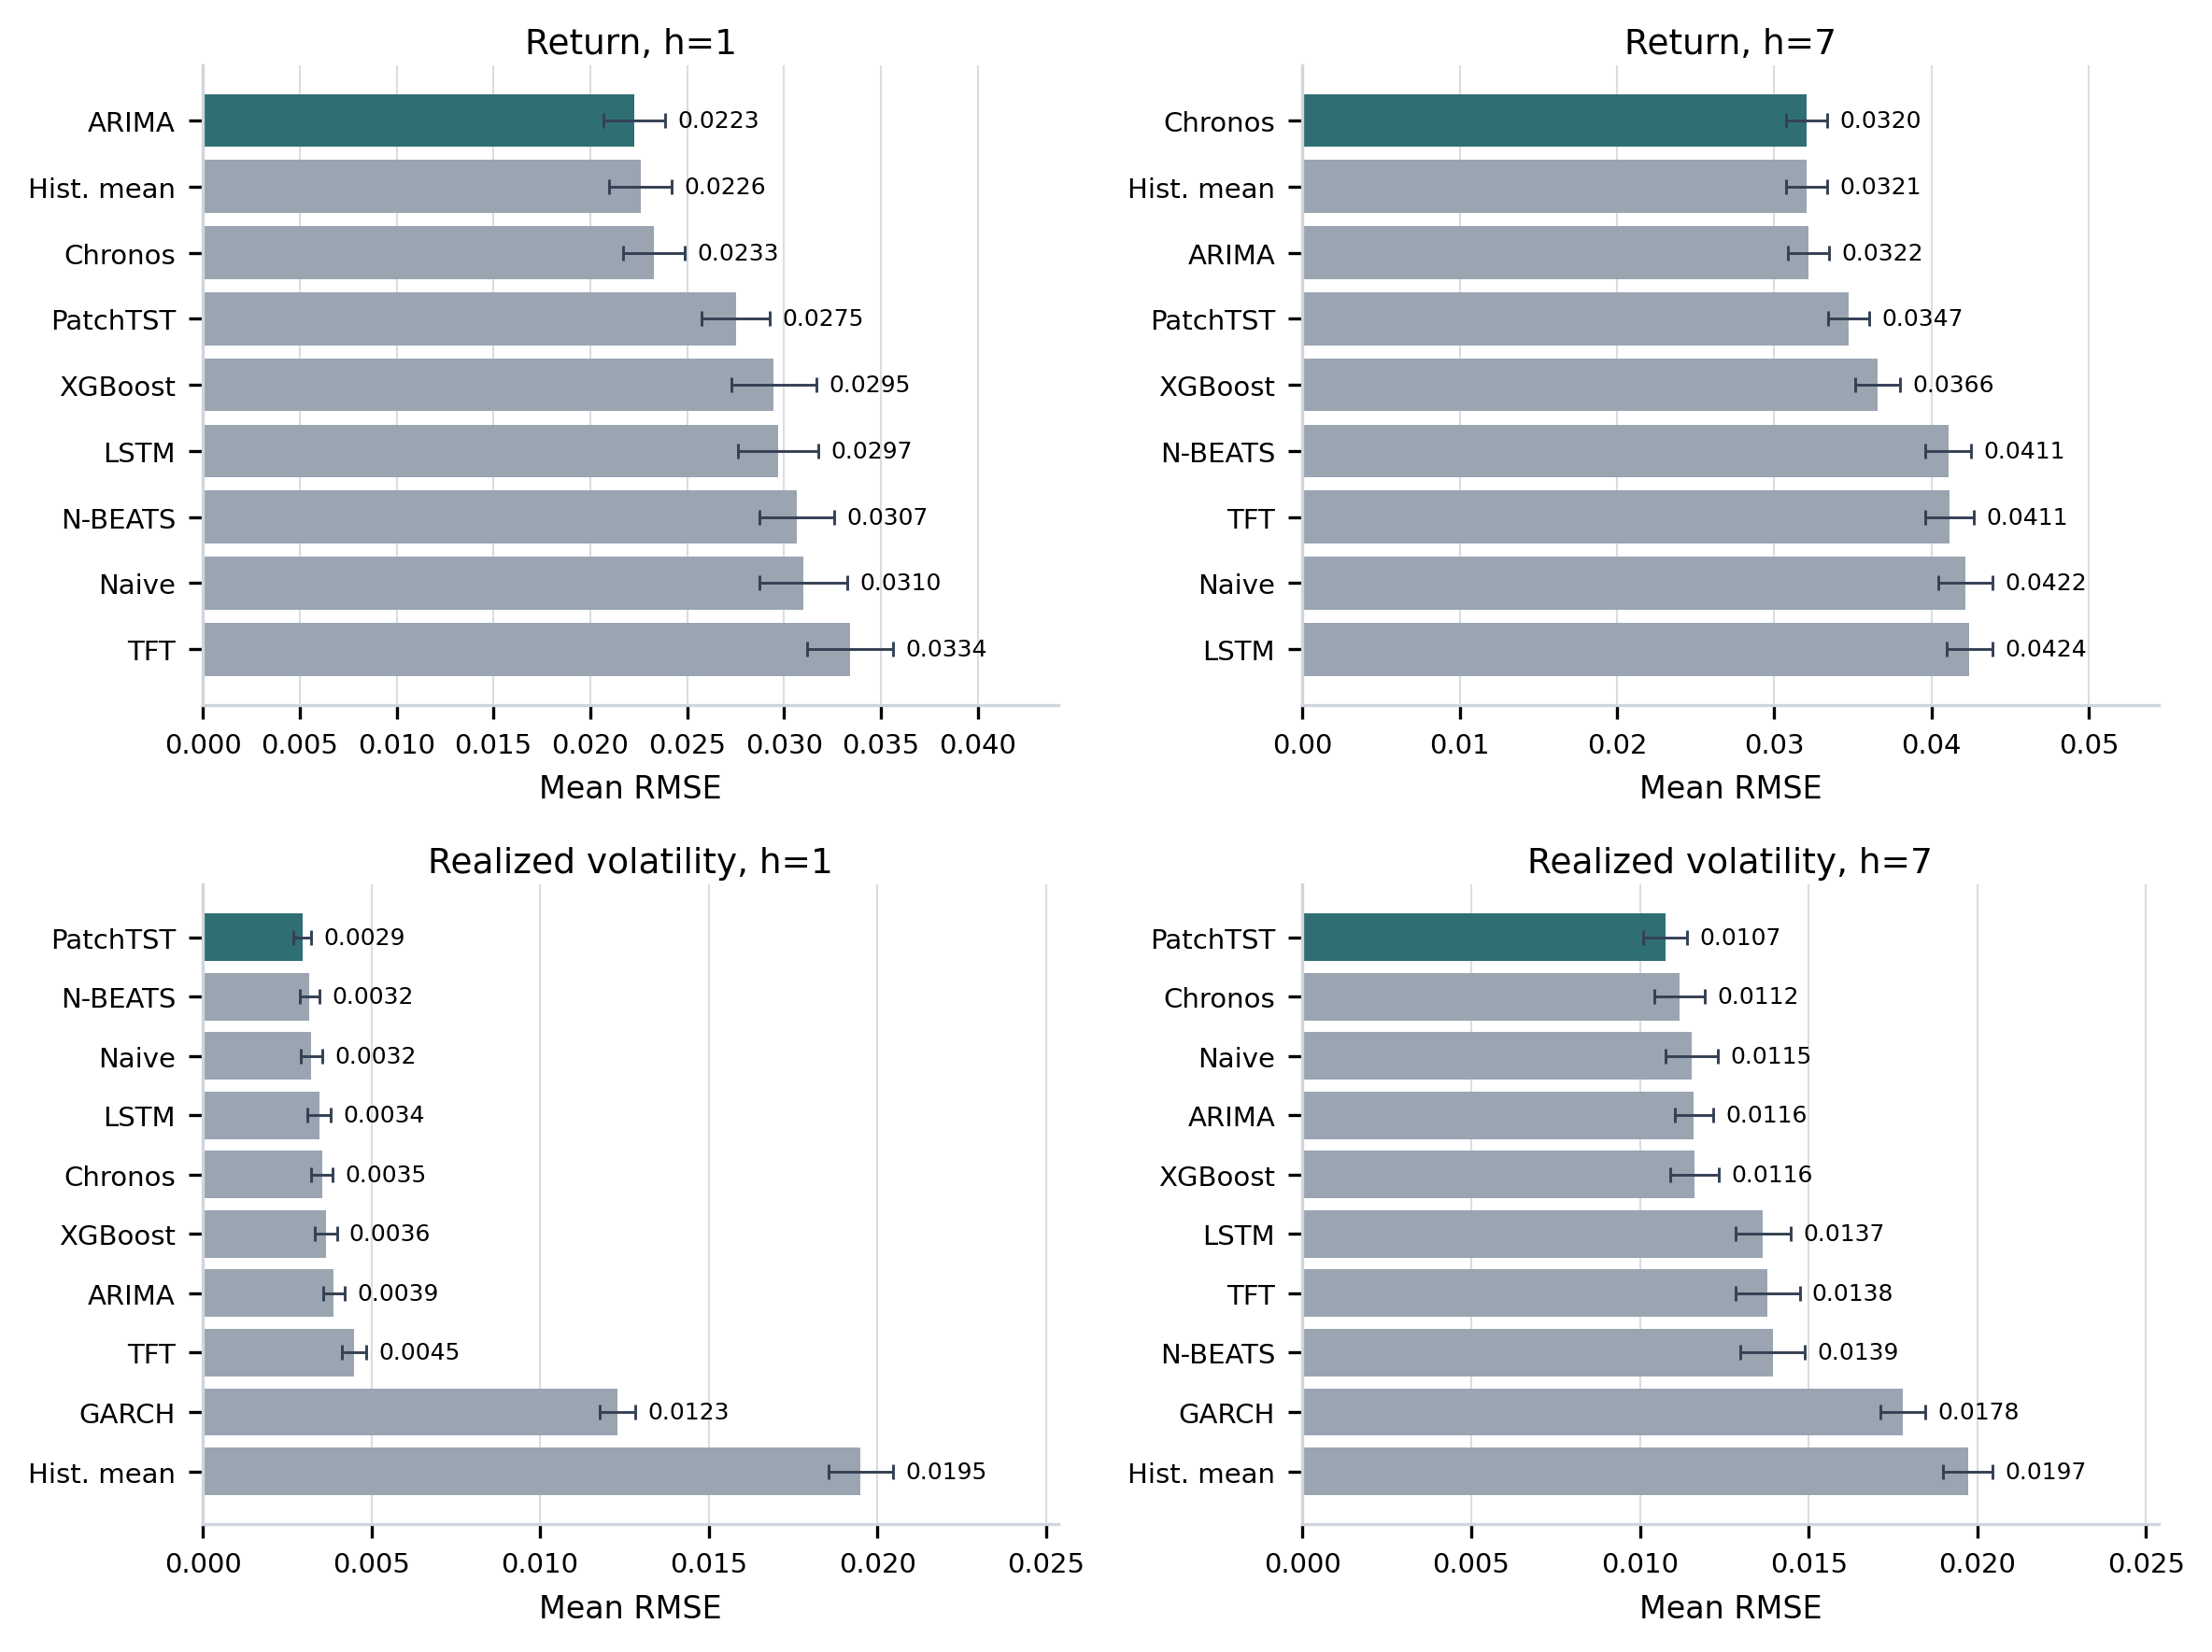
\includegraphics[width=0.95\textwidth]{figures/rmse_overview.png}
\caption{Mean RMSE across all walk-forward asset-splits. Error bars show one
standard error of the mean; the best model in each panel is highlighted.}
\label{fig:rmse}
\end{figure*}

For realized volatility, PatchTST is the strongest model by mean RMSE at both
horizons. At one day it is followed by N-BEATS and naive persistence. At seven
days it is followed by Chronos, naive persistence, ARIMA, and XGBoost, all of
which are tightly clustered. Mean-rank analysis is consistent with this
pattern: naive persistence has the best average RMSE rank for one-day
volatility, while PatchTST has the best average RMSE rank for seven-day
volatility.

Diebold-Mariano tests reinforce the cautious interpretation. For one-day
returns, ARIMA is significantly better than naive persistence and PatchTST, but
not significantly different from historical mean or Chronos. For seven-day
returns, Chronos is significantly better than PatchTST, XGBoost, and naive
persistence, but not significantly different from historical mean or ARIMA.
For one-day volatility, PatchTST is significantly better than naive
persistence, N-BEATS, Chronos, ARIMA, and XGBoost at the 5\% level. For
seven-day volatility, PatchTST is significantly better than N-BEATS, LSTM, and
TFT, but not significantly different from Chronos, naive persistence, ARIMA,
or XGBoost. Directional accuracy for returns remains close to chance, with the
best values near 0.57 for one-day returns and 0.52 for seven-day returns,
again suggesting that point-error gains do not directly translate into
reliable directional trading signals.

\section{Discussion}
The full benchmark supports the main thesis with a more precise interpretation.
Modern neural forecasters are not a universal solution for cryptocurrency
returns, because classical baselines remain extremely competitive and
directional accuracy remains close to chance. The strong performance of the
historical-mean baseline is theoretically consistent with this setting: if
daily returns are close to zero-drift noise, predicting the historical mean is
near-optimal under squared-error loss. Neural forecasters are more useful
competitors for volatility forecasting, where PatchTST produces clear and
statistically significant gains at the one-day horizon and a smaller,
less statistically distinguished numerical lead at seven days. Chronos is also
notable because it is competitive without asset-specific fine-tuning and is
strongest for seven-day return RMSE in this benchmark.

\section{Conclusion}
We introduced a reproducible walk-forward benchmark for cryptocurrency return
and volatility forecasting. In the full benchmark, ARIMA remains strongest for
one-day returns, Chronos is marginally strongest for seven-day returns, and
PatchTST shows clear gains on one-day realized volatility, with a smaller and
less statistically distinguished lead at the seven-day horizon. The broader
lesson is methodological: in crypto forecasting, careful validation and strong
baselines matter as much as model class. Our scope is intentionally narrow:
daily data on five major assets, point forecasts only, and zero-shot use of one
foundation model. Generalization to intraday horizons, larger asset universes,
fine-tuned foundation models, and probabilistic evaluation remains open. Future
work will add volatility-regime error analysis and include probabilistic scores
for models that produce predictive distributions.

\section*{Acknowledgments}
Acknowledgments will appear in the camera-ready version.

\FloatBarrier
\bibliographystyle{ICICPEtran}
\bibliography{references}

\end{document}
